\chapter{Comparison of MOR Methods} \label{analysis}
The previously mentioned methods for model order reduction will be compared regarding time domain error, frequency domain error and computational speed.
The time domain error will be obtained by comparing the FEM solution to a given approximation.
To get insights into the frequency domain error, the error system of a reduced order model will be analysed.
The computational speed will be determined by measuring the time it takes to generate a ROM.
Here it is assumed that the implementations provided by MORLAB are programmed in a sufficiently effective manner.
For testing the following parameters are used
\begin{gather}
\alpha = 0.1, \quad T = 1, \quad L = 1 \\
n = 100, \quad n_t = 10^{4}
\end{gather}
.

These values are chosen such that it yields results in a timely manner.
Especially \(n_t\) and \(\alpha\) are important for stability of euler scheme.
If both are too low, the euler scheme becomes unstable.
Choosing \(n_t\) too high the time and memory consumption becomes rather large.
There was no exact method for determining the parameters in this way.

\section{Time Domain Error}
The time domain error will defined as \(\epsilon = Y - \hat{Y}\) where \(Y\) and \(\hat{Y}\) denote the matrices storing the output of the systems \(G\) and \(G_r\).
Since the output matrices are usually rather large, it is impractical to use \(\epsilon\) directly.
Therefore  \(||\epsilon||_{max}\)  and \(||\epsilon||_{F}\) as well as \(\epsilon\) will be considered.
The maximum norm will be used to show the magnitude of the worst occurring error.
Since this is susceptible to spikes the error is also measured using the Frobenius norm to get a measure of the error that respects all data points.
Here two aspects are interesting.
The first one is how the errors behaves as \(r\) gets larger and the second aspect is how the error evolves over time for some fixed \(r\).
To get data about the first aspect \(||\epsilon||_{max}\)  and \(||\epsilon||_{F}\) will be measured for increasing \(r\).
Data about the second aspect will be gathered by calculating the norm of the error between the column vectors of \(Y\) and \(\hat{Y}\) for some fixed \(r\), \(\epsilon_{t} = ||Y_t - \hat{Y}_t||_{2}\) where \(A_t\) denotes the \(t^{th}\) column vector of \(A\).
Since here vectors are compared the euclidean norm is used since it is compatible to the Frobenius norm.
The Chebychev norm can also be used as vector norm.
There will be two different initial conditions considered.
The first one is \(x(0, x) = 1\).
It is chosen in this way to display the workings of the boundary condition.
If there were no boundary conditions, for a constant initial condition the system would never cool down since \(\frac{\partial^2 u}{\partial x^2} = 0\) (\ref{eq-1d-h}) at every point in time.
This only holds if there is no input to the system.
Therefore \(u(t) = 0\), where \(u\) denotes the systems input.
The second initial condition is \(x(0, x) = 4\sin(\frac{2\pi}{L}x)\) with random input.
The initial condition is sinusoidal since it is easy to approximate.
The input is random to show the error of the models if the inputs are erratic.
\subsection{Absolute error}
\paragraph{Proper Orthogonal decomposition}
\begin{figure}
\centering
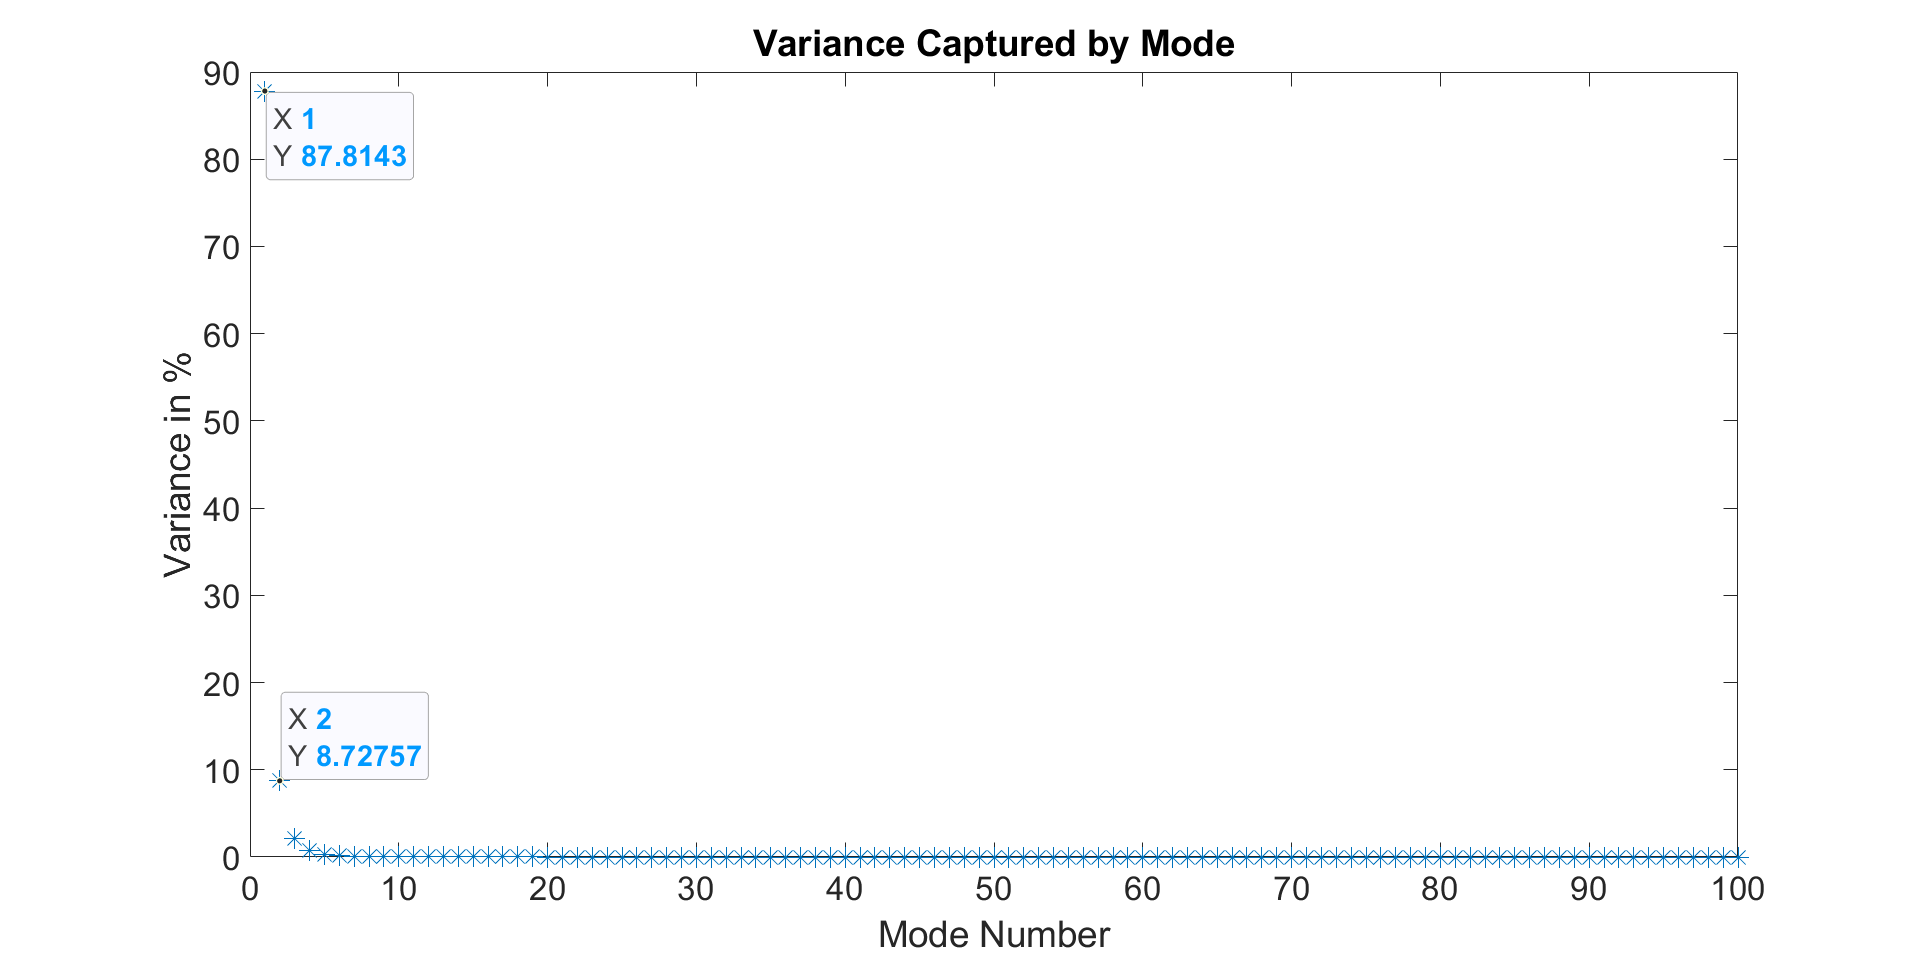
\includegraphics[ width=\textwidth]{images/test_modes_pod}
\label{Variance captured by POD Modes}
\label{FIG-POD-MODES}
\end{figure}


\begin{figure}[H]
\begin{subfigure}{.5\textwidth}
\centering
\includegraphics[ width=7.5cm]{images/abs\_Proper Orthorgonal Decomposition\_10\_100}
\caption{Absolute error POD, var=10\%}
\label{FIG-ABS-POD10}
\end{subfigure}
\begin{subfigure}{.5\textwidth}
\centering
\includegraphics[ width=7.5cm]{images/abs\_Proper Orthorgonal Decomposition\_25\_100}
\caption{Absolute error POD, var=25\%}
\label{FIG-ABS-POD25}
\end{subfigure}
\caption{Absolute error POD, var=10\% and var=25\%}
\label{FIG-ABS_POD1}
\end{figure}


\begin{figure}[H]
\begin{subfigure}{.5\textwidth}
\centering
\includegraphics[ width=7.5cm]{images/abs\_Proper Orthorgonal Decomposition\_50\_100}
\caption{Absolute error POD, var=50\%}
\label{FIG-ABS-POD50}
\end{subfigure}
\begin{subfigure}{.5\textwidth}
\centering
\includegraphics[ width=7.5cm]{images/abs\_Proper Orthorgonal Decomposition\_75\_100}
\caption{Absolute error POD, var=75\%}
\label{FIG-ABS-POD75}
\end{subfigure}
\caption{Absolute error POD, var=50\% and var=75\%}
\label{FIG-ABS_POD2}
\end{figure}

\begin{figure}[H]
\begin{subfigure}{.5\textwidth}
\includegraphics[ width=7.5cm]{images/abs\_Proper Orthorgonal Decomposition\_99\_100}
\caption{Absolute error POD, var=99\%}
\label{FIG-ABS-POD100}
\end{subfigure}
\begin{subfigure}{.5\textwidth}
\centering
\includegraphics[ width=7.5cm]{images/abs\_Proper Orthorgonal Decomposition\_100\_100}
\caption{Absolute error POD, var=100\%}
\label{FIG-ABS-POD100}
\end{subfigure}
\caption{Absolute error POD, var=99\% and var=100\%}
\label{FIG-ABS_POD3}
\end{figure}
